\subsection{Docker-Compose Layer Diagram}
\label{subsec:docker_compose_diagram}
This section illustrates the different layers of the docker-compose 
containers based on the way it was used in the 
deployment of the system.
\hfill \\

Figure \ref{fig:docker_compose_layout} shows a diagram based
on Docker documentation, to better understand the containers and layers
of the alamSYS. \textit{Note that in the diagram the lowest level is the "Server Infrastructure"
and the highest level is the "Docker-Compose" layer.}
% Docker-Compose Layer Diagram
\begin{figure}[ht]
    \centering
    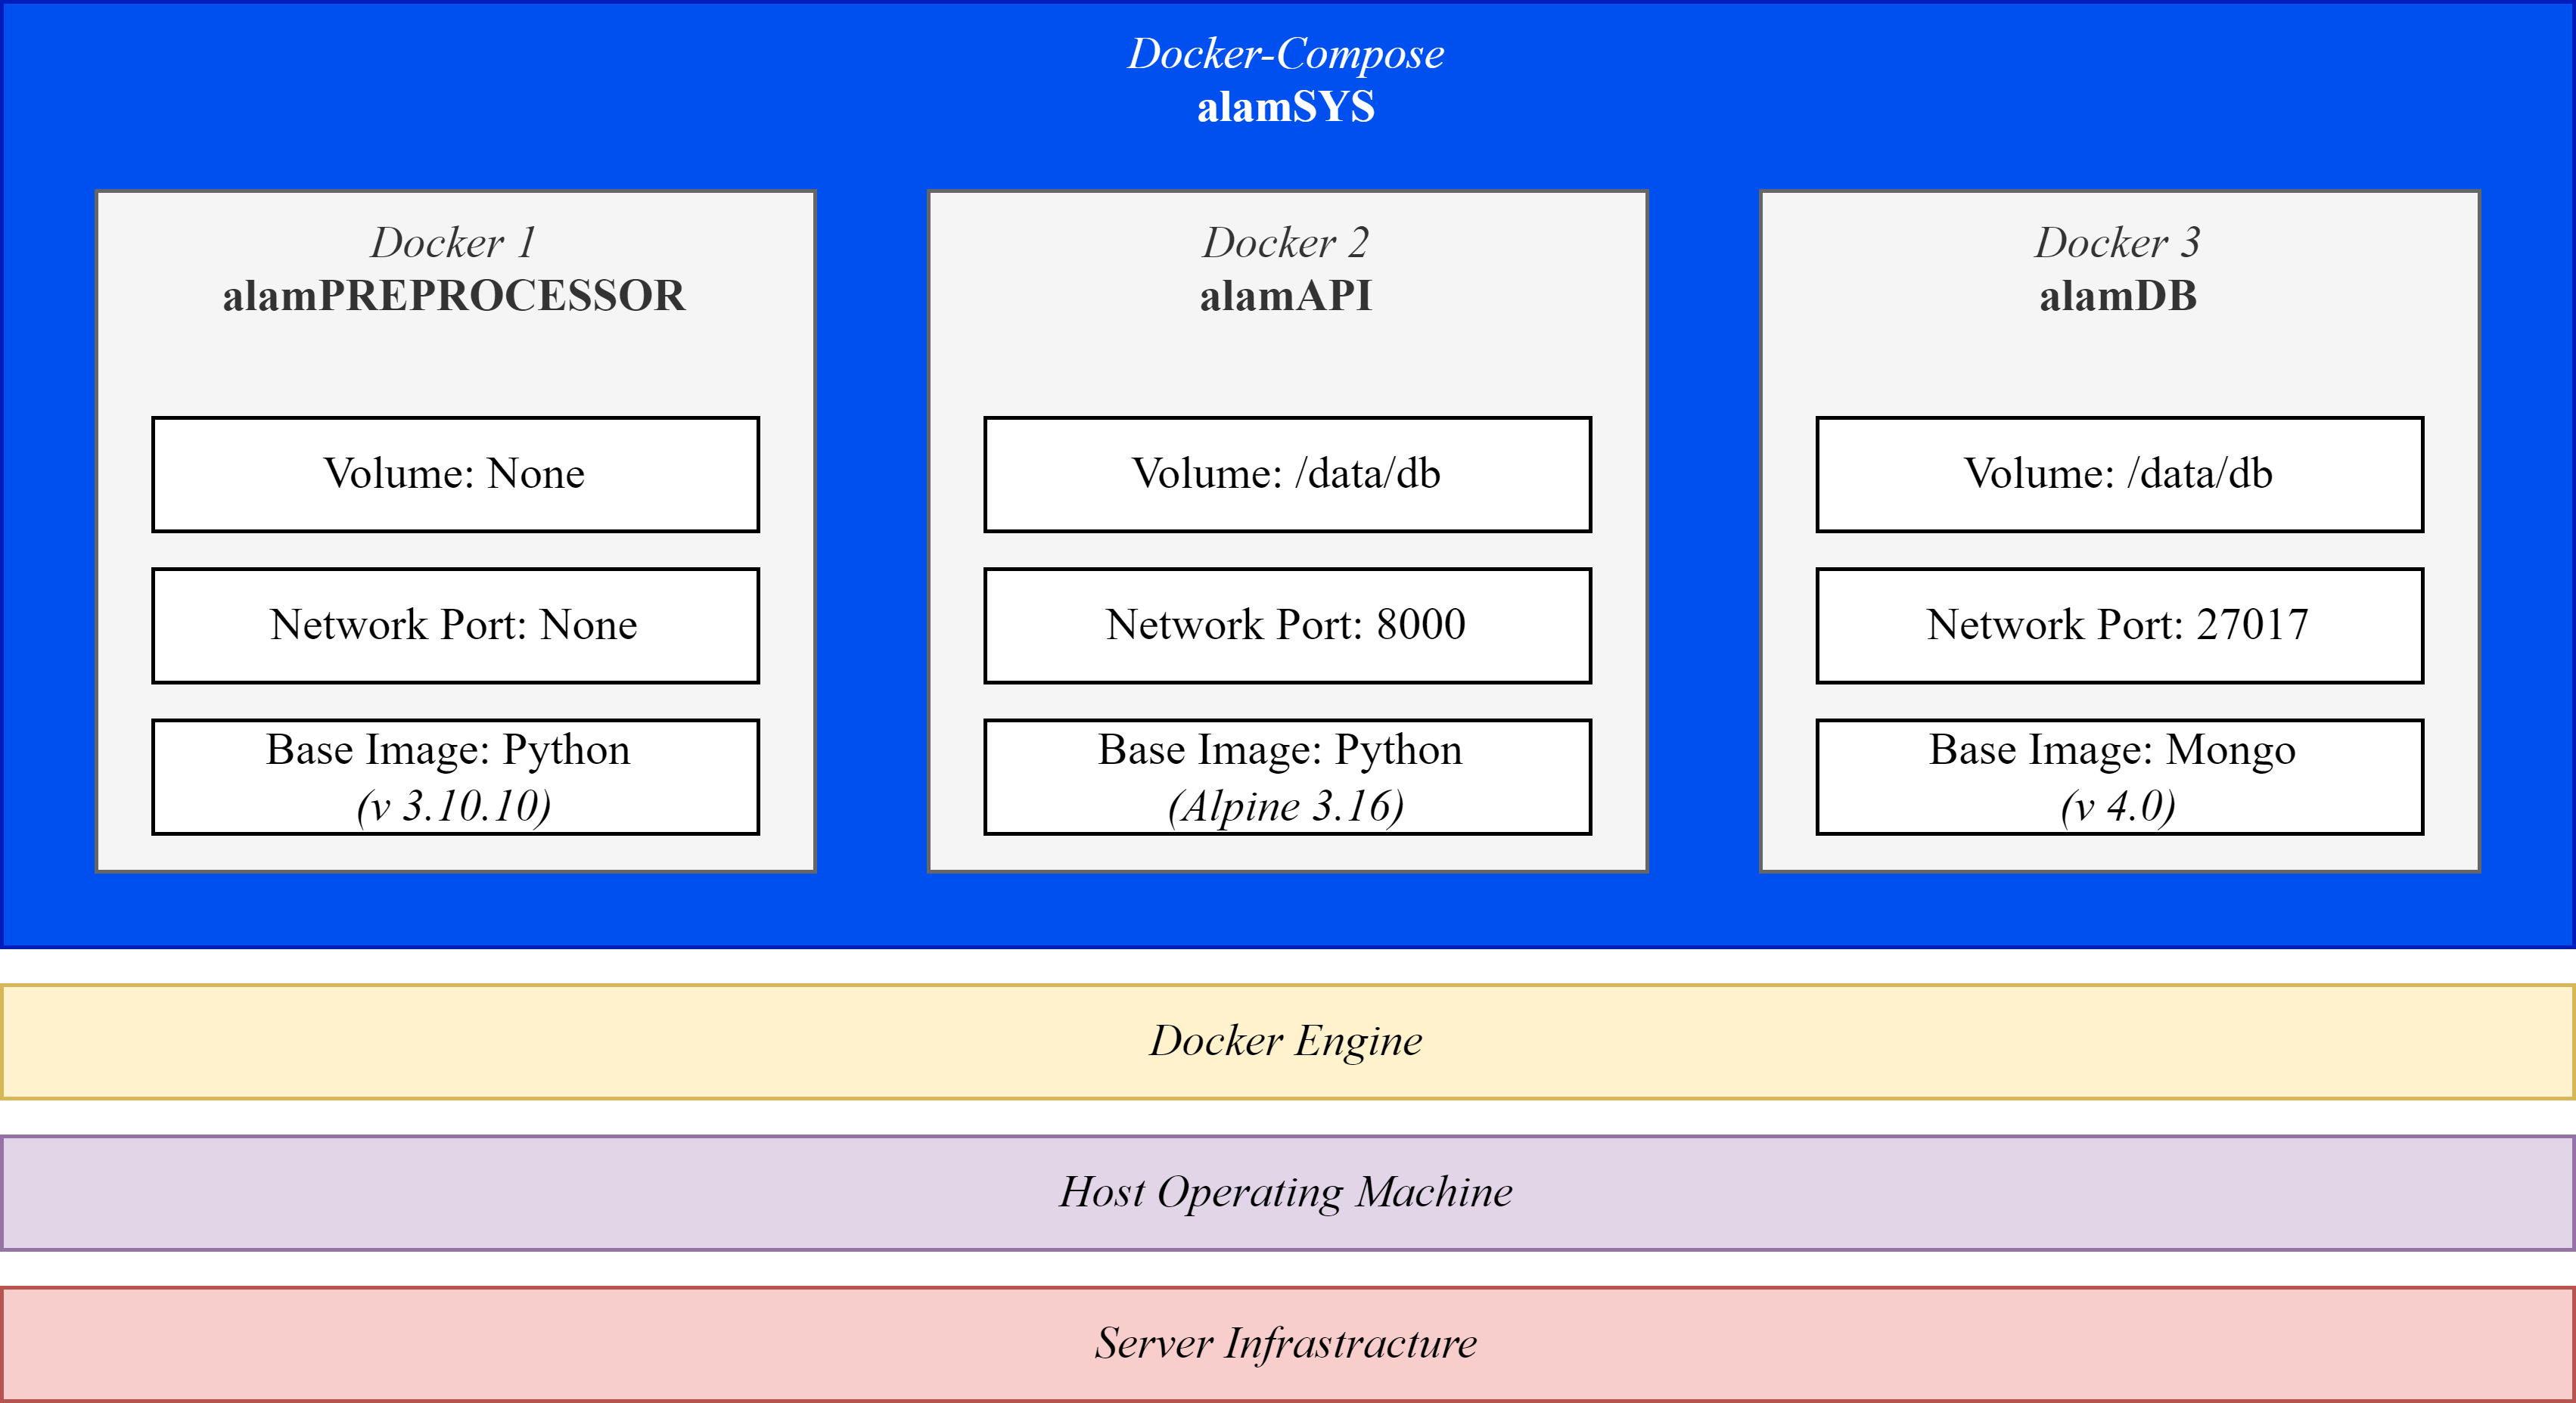
\includegraphics[width=1\textwidth]{./assets/Chapter_3/Docker-Compose Layout.png}
    \caption{Docker-Compose Layer Diagram for the alamSYS}
    \label{fig:docker_compose_layout}
\end{figure}
\FloatBarrier

From the figure above, it can be observed that the docker-compose layer is composed
of three docker containers, which are as follows:
\begin{itemize}
    \item[(a)] Docker 1 : alamPREPROCESSOR - This is the docker container that contains
    the alamPREPROCESSOR application. It uses Python 3.11.2 as its based image. Moreover,
    this container is connected to the data/db volume, and there is no network port exposed.
    \item[(b)] Docker 2 : alamAPI - This is the docker container that contains the alamAPI
    application. It uses a Python image as well, but is running on top of an Alpine 3.16 image.
    This was done as Alpine images runs on minimal resources than other Linux based images.
    Furthermore, it is not attached to any volume, and its network port
    8000 is exposed.
    \item[(c)] Docker 3 : alamDB - This is the docker container that contains the alamDB application
    which runs on top of the Mongo version 4.0 image. Similarly to alamPREPROCESSOR, it is also 
    connected to the data/db volume, while its network port 27017 is exposed.
\end{itemize}